\documentclass[a4paper, fleqn]{article}
\usepackage{header}

\usetikzlibrary{patterns}
\usepgfplotslibrary{fillbetween}

\title{Семинарский лист 2.3}
\author{
    Александр Богданов   \\ \href{https://t.me/SphericalPotatoInVacuum}{Telegram} \and
    Алиса Вернигор       \\ \href{https://t.me/allisyonok}{Telegram} \and
    Анастасия Григорьева \\ \href{https://t.me/weifoll}{Telegram} \and
    Василий Шныпко       \\ \href{https://t.me/yourvash}{Telegram} \and
    Данил Казанцев       \\ \href{https://t.me/vserosbuybuy}{Telegram} \and
    Денис Козлов         \\ \href{https://t.me/DKozl50}{Telegram} \and
    Елизавета Орешонок   \\ \href{https://t.me/eaoresh}{Telegram} \and
    Иван Пешехонов       \\ \href{https://t.me/JohanDDC}{Telegram} \and
    Иван Добросовестнов  \\ \href{https://t.me/ivankot13}{Telegram} \and
    Настя Городилова     \\ \href{https://t.me/nastygorodi}{Telegram} \and
    Никита Насонков      \\ \href{https://t.me/nnv_nick}{Telegram} \and
    Сергей Лоптев        \\ \href{https://t.me/beast_sl}{Telegram}
}

\date{Версия от {\ddmmyyyydate\today} \currenttime}

\begin{document}
    \maketitle
    
    \section*{Предполагая функцию $f$ непрерывной на $D$, приведите двойной интеграл от $f$ по $D$ к повторному 
    двумя способами: по $x$ затем по $y$ и наоборот.}
    \subsection*{Задача 1\\[-40 pt]}
    \begin{align*}
        & D = \{ (x, y) \,|\, x, y \in [0; 1], x^2 + y^2 \ge 1 \} \\[3 pt]
        & \text{Множество точек, находящихся в квадрате, ограниченном прямыми $x = 0, x = 1, y = 0, y = 1$,} \\
        & \text{за пределами круга радиуса 1 с центром в точке $(0, 0)$:} \\[3 pt]
        & \text{Интеграл по $x$ затем по $y$:} \\
        & \int\limits_0^1 dy \!\!\! \int\limits_{\sqrt{1-y^2}}^1 \!\!\! dx = \int\limits_0^1 dy \cdot x \Bigm|_{\sqrt{1-y^2}}^1
        = \int\limits_0^1 dy \left( 1 - \sqrt{1-y^2} \right) = \int\limits_0^1 dy - \int\limits_0^1 \sqrt{1-y^2} \, dy 
        = 1 - \int\limits_0^1 \sqrt{1-y^2} \, dy \\
        & \text{Замена: } y = \sin u \Leftrightarrow \int\limits_0^1 \sqrt{1-y^2} \, dy 
        = \int\limits_0^{\frac{\pi}2} \cos u \, \sqrt{1-\sin^2 u} \, du = \int\limits_0^{\frac{\pi}2} \cos^2 u \, du 
        = \int\limits_0^{\frac{\pi}2} \frac{\cos 2u + 1}2 \, du = \\
        & = \frac12 \int\limits_0^{\frac{\pi}2} \cos 2u \, du + \frac12 \int\limits_0^{\frac{\pi}2} \! du 
        = \frac14 \, \sin 2u \Bigm|_0^{\frac{\pi}2} + \frac12\, u \Bigm|_0^{\frac{\pi}2} = \frac{\pi}4 \\
        & \text{Тогда:} \\
        & \int\limits_0^1 dy \!\!\! \int\limits_{\sqrt{1-y^2}}^1 \!\!\! dx = 1 - \frac{\pi}4 \\
        & \text{Очевидно, что повторный интеграл, взятый в другом порядке, будет вычисляться точно так же:} \\
        & \int\limits_0^1 dx \!\!\! \int\limits_{\sqrt{1-x^2}}^1 \!\!\! dy = \int\limits_0^1 dy \cdot y \Bigm|_{\sqrt{1-x^2}}^1
        = \int\limits_0^1 dx \left( 1 - \sqrt{1-x^2} \right) = \int\limits_0^1 dy - \int\limits_0^1 \sqrt{1-x^2} \, dy 
        = 1 - \frac{\pi}4 \\
        & \text{\fbox{Ответ: $1 - \dfrac{\pi}4$.}}
    \end{align*}
    
    \subsection*{Задача 2\\[-40 pt]}
    \begin{align*}
        & D = \{ (x, y) \,|\, x, y \in [0; 1], (x - 1)^2 + (y - 1)^2 \ge 1 \} \\[3 pt]
        & \text{Множество точек, находящихся в квадрате, ограниченном прямыми $x = 0, x = 1, y = 0, y = 1$,} \\
        & \text{за пределами круга радиуса 1 с центром в точке $(1, 1)$:} \\[3 pt]
        & \text{Интеграл по $x$ затем по $y$:} \\
        & \int\limits_0^1 dy \!\!\! \int\limits_0^{\sqrt{1-(y-1)^2}+1} \!\!\! dx 
        = \int\limits_0^1 dy \cdot x \Bigm|_0^{\sqrt{1-(y-1)^2}+1} = \int\limits_0^1 dy \left( \sqrt{1-(y-1)^2} + 1 \right) 
        = \int\limits_0^1 \sqrt{1-(y-1)^2} \, dy + 1 \\
        & \text{Замена: } (y-1) = \sin u \Leftrightarrow \int\limits_0^1 \sqrt{1-(y-1)^2} \, dy 
        = \int\limits_0^{\frac{\pi}2} \cos u \, \sqrt{1-\sin^2 u} \, du = \int\limits_{-\frac{\pi}2}^0 \cos^2 u \, du 
        = \int\limits_{-\frac{\pi}2}^0 \frac{\cos 2u + 1}2 \, du = \\
        & = \frac12 \int\limits_{-\frac{\pi}2}^0 \cos 2u \, du + \frac12 \int\limits_{-\frac{\pi}2}^0 \! du 
        = \frac14 \, \sin 2u \Bigm|_{-\frac{\pi}2}^0 + \frac12\, u \Bigm|_{-\frac{\pi}2}^0 = -\frac{\pi}4 \\
        & \text{Тогда:} \\
        & \int\limits_0^1 dy \!\!\! \int\limits_0^{\sqrt{1-(y-1)^2}+1} \!\!\! dx = 1 - \frac{\pi}4 \\
        & \text{Очевидно, что повторный интеграл, взятый в другом порядке, будет вычисляться точно так же:} \\
        & \int\limits_0^1 dx \!\!\! \int\limits_0^{\sqrt{1-(x-1)^2}+1} \!\!\! dy = \int\limits_0^1 \sqrt{1-(x-1)^2} \, dx + 1
        = 1 - \frac{\pi}4 \\
        & \text{\fbox{Ответ: $1 - \dfrac{\pi}4$.}}
    \end{align*}
    
    % \subsection*{Задача 3}
    
    % \subsection*{Задача 4}
    
    \section*{Предполагая функцию $f$ непрерывной на $D$, измените порядок интегрирования в повторном интеграле}
    % \subsection*{Задача 5}

    \subsection*{Задача 6}
    \begin{flalign*}
        & \int_0^1 dy \int_{\frac{y^2}{9}}^{y} f(x, y) dx + 
        \int_1^3 dy \int_{\frac{y^2}{9}}^1 f(x, y) dx = \text{ пристально смотрим на рисунок } = \\
        & = \int_0^1 \int_{x}^{3\sqrt{x}} f(x, y) dx dy = 
        \int_0^1 dx \int_{x}^{3\sqrt{x}} f(x, y) dy 
    \end{flalign*}
    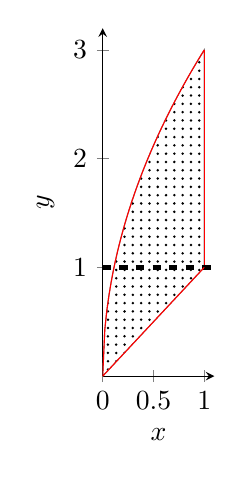
\begin{tikzpicture} 
        \begin{axis}[axis lines=center, xlabel={$x$}, ylabel={$y$}, % служебные строки
                        xlabel near ticks, ylabel near ticks, hide obscured x ticks=false, % служебные строки
                        xmin=0, xmax=1.1, ymin=0, ymax=3.2, % диапазон значений
                        width=3cm, height=6cm] % размер картинки
            % чтобы рисовать линии по координатам (x, y) используйте (axis cs:x, y), как здесь:
            \draw[color=red] (axis cs:1, 1) -- (axis cs:1, 3); % вертикальная линия справа
            \draw[dashed, line width=2pt, color=black] (axis cs:0, 1) -- (axis cs:1.1, 1); % деление двух интегралов
            % чтобы заполнить площадь между графиками стоит дать графикам имена (здесь A и B):
            \addplot [name path=A, domain=0:1, color=red] {x}; 
            \addplot [name path=B, domain=0:1, color=red, samples=50] {sqrt(x)*3}; % тикз умеет в математику
            \addplot [pattern=dots, draw=gray] fill between[of=A and B]; % само заполнение через fill between
        \end{axis} 
    \end{tikzpicture} 

    % \subsection*{Задача 7}
    
    % \subsection*{Задача 8}
    
    \section*{Изменив порядок интегрирования, вычислите интеграл}
    % \subsection*{Задача 9}
    
    \subsection*{Задача 10}
    
    % \subsection*{Задача 11}
    
    % \subsection*{Задача 12}
    
    \section*{Вычислите интеграл}
    % \subsection*{Задача 13}
    
    \subsection*{Задача 14}
    
    % \subsection*{Задача 15}
    
    % \subsection*{Задача 16}
    
    \section*{Предполагая функцию $f$ непрерывной на $D$, измените порядок интегрирования в повторном интеграле
    всеми возможными способами}
    % \subsection*{Задача 17}
    
    \subsection*{Задача 18}
    
    % \subsection*{Задача 19}
    
    % \subsection*{Задача 20}
    
    % \subsection*{Задача 21}
    
    % \subsection*{Задача 22}
    
\end{document}
